\documentclass{article}

\usepackage{polyglossia}
\usepackage{xcolor}
\usepackage{fontspec}
\usepackage{mathtools}
\usepackage{graphicx}
\setdefaultlanguage{french}
\setlength{\parskip}{4pt}
\newtheorem{definition}{Définition}

\begin{document}

\section{Introduction}

\subsection{Trois points de vue sur la notation objet}

\begin{itemize}
	\item Abstraction (type abstrait) - point de vue structure
		\begin{itemize}
			\item Cache les structures (ex: pile) par les manipulations légales (ex: empiler,
				dépiler)
			\item On parle \emph{d'encapsulation} de l'objet
		\end{itemize}
	\item Réseaux sémantiques (Intelligence artificielle) - point de vue concept
	\begin{itemize}
		\item Sous classe SC \emph{est une sorte de classe} C
		\item Objet O \emph{est un (est une instance)} de C
	\end{itemize}
	\item Langage d'acteurs (Intelligence artificielle) - point de vue dynamique
	\begin{itemize}
		\item l'objet O reçoit un message et y réagit
		\item Système multi-agents
	\end{itemize}
\end{itemize}

\subsection{Trois grandes classes d'applications}

\begin{itemize}
	\item La conception = représenter le monde réel pour l'informatiser
	\begin{itemize}
		\item Représente les entités (classe) et les liens (héritage) naturellement
		\item Visualisation facile (graphe des classes), synthèse et modifications
	\end{itemize}
	\item La programmation = le codage
	\begin{itemize}
		\item La programmation jaillit de la modélisation
		\item Les fonctions sont relatives aux données
		\item Un même nom de fonction pour même opération, même si codage
			différent (langage abstrait)
	\end{itemize}
	\item Les bases de données = la persistance
	\begin{itemize}
		\item Pourquoi utiliser des tables ?
		\item Objets persistants
	\end{itemize}
\end{itemize}

\subsection{Principes}

\begin{itemize}
\item Principe 1 : on raccroche à la structure de données (champs),
	les codes qui peuvent les manipuler (méthode) -> classe
\item Principe 2 : on hiérarchise les classes -> héritage
\item Principe 3 : on assure la sécurité des accès aux données et
	méthodes sous forme d’autorisation; on gère les erreurs
\end{itemize}

\section{Propriétés des accès}
Qui peut accéder aux champs, méthodes et classes ?

\subsection{Le constructeur}
\begin{itemize}
	\item Appliqué à une classe retourne un objet de la classe
	\begin{itemize}
		\item Créer un objet à partir d'une classe
		\item Initialiser l'objet par les valeurs adéquates (initialiser 
		après le new les champs)
	\end{itemize}
	\item Programmer des constructeurs paramétrés
	\begin{itemize}
		\item (LOLO): nomClasse <= new(val1,..,valn)
		\item (en JAVA): définir des méthodes du nom de la classe
		\begin{itemize}
			\item Quand aucun constructeur n'est défini -> constructeur par défaut
			\item Le constructeur par défaut est désactivé dès qu'il existe un 
				constructeur programmé
			\item On peut reconstruire à la main un constructeur sans paramètre
		\end{itemize}
	\end{itemize}
	\item L'utilisation de \emph{super}
	\begin{itemize}
		\item super() appel le constructeur de la sur-classe
		\item super.méthode(\dots) appel de méthode de la classe supérieur
	\end{itemize}
\end{itemize}

\subsection{Accès privé/public}

L'accès à un champs peut être : 
\begin{itemize}
	\item \textbf{privé} : seules les méthodes de la classe C peuvent utiliser
		le champs
	\item \textbf{public} : tout code (ayant accès à la classe C) peut l’utiliser
	\item \textbf{protégé} : seules les méthodes de la classe C et de ses sous
		classes peuvent utiliser le champs
\end{itemize}

Règles :
\begin{itemize}
	\item un champs est généralement privé
	\item --> accès par des méthodes adéquates
	\item un champs gérant des données d'implémentation est privé
\end{itemize}

L'accès aux méthodes m d'une classe C peut être :
\begin{itemize}
	\item \textbf{privé} : seules les méthodes de la classe C peuvent utiliser m
	\item \textbf{public} : tout code (ayant accès à la classe C) peut utiliser m
	\item \textbf{protégé} : seules les méthodes de la classe C et de ses sous classes
		peuvent utiliser m 
\end{itemize}

Remarques :
\begin{itemize}
	\item \emph{private, public, protected} (en JAVA) sont appelés des
modificateurs (d'accès)
	\item Accesseurs (conventions)
	\begin{itemize}
		\item \emph{getVar} : accès lecture à un champs \emph{Var}
		\item \emph{setVar} : accès écriture à un champs \emph{Var}
	\end{itemize}
\end{itemize}

On parle de portée d'une déclaration

\subsection{Les paquetages}

Un paquetage, en JAVA, n'existe pas en Smalltalk ou C++

\begin{itemize}
	\item Idées
	\begin{itemize}
		\item pour de grandes applications
		\item regroupe des classes dans un paquetage (\emph{package} en JAVA)
		\item Nom de la classe, référé à un paquetage (permet 2 classes de même nom)
		\item  Les paquetages organisent logiquement les classes dans une hiérarchie;
	généralement, l’organisation physique est la même
	\end{itemize}
	\item Principes du package (logique) et de son positionnement système (physique)
	\begin{itemize}
		\item Un package est associé à un répertoire : le nom du pakage est celui du
			répertoire
		\item Une hiérarchie de packages correspond à une hiérarchie de répertoires
		\item Dans un package, il y a des classes, et des sous packages (= sous répertoires)
		\item Le premier niveau de hiérarchie correspond au nom de l’application ou du
			propriétaire (ex: loiseau, java)
	\end{itemize}
	\item Principes de nommage, d’appartenance et de recherche
	\begin{itemize}
		\item un mécanisme de nommage : \emph{nomPackage.nomSousPackage.NomClasse}
		\item appartenance :
			\begin{itemize}
				\item Par défaut: une classe dans un répertoire appartient au package 
					correspondant
				\item Par déclaration: package nomPackage.nomSousPackage (1ere instr)
			\end{itemize}
		\item recherche : variable \emph{CLASSPATH} (Windows)
	\end{itemize}
	\item Accès aux classes d’un package
	\begin{itemize}
		\item les classes \emph{(object, String...)} du package \emph{java.lang} sont utilisables
			dans toute classe
		\item pour importer une classe C ou un packetage P dans un programme :
			\emph{import C} et \emph{import P.* } en tête de fichier
		\item Si pas de modificateur de champs et méthode: toutes les classes du package y
			ont accès
		\item Attention : Modificateur d'accès d'une classe C,  
			\emph{public} : la classe est accessible en dehors du package où elle est définie
			pas de modificateur: seules les classes du même paquetage ont accès à C
	\end{itemize}
\end{itemize} 

\section{Les classes pour elles-même}

\subsection{Retour à l'héritage}

\begin{itemize}
	\item l'autoréférencement
	\begin{itemize}
		\item pour appliquer une méthode à l'objet
		\item pour lever l'ambiguïté entre nom de champs et variable
	\end{itemize}
	\item L'option \emph{final} (sécurité)
	\begin{itemize}
		\item une méthode \emph{final} ne peut pas être redéfinie dans une sous classe
		\item une classe définie \emph{final} ne peut pas être héritée
		\item une variable \emph{final} est une constante
	\end{itemize}
\end{itemize}

\subsection{Classe abstraite}

\begin{definition}
	Une classe abstraite est une classe pour laquelle il ne peut
exister d'instances.
\end{definition}

\begin{itemize}
	\item elle factorise les champs et méthodes de sous classes
	\item elle est déclarée avec le mot clef \emph{abstraite (abstract)}
\end{itemize}

\begin{definition}
	Une méthode abstraite d'une classe C est une méthode ne
possédant pas de corps. La méthode doit être implémentée dans chaque
sous-classe de la classe C
\end{definition}

\begin{itemize}
	\item elle est redéfinie au niveau des sous classes
	\item vérification à la compilation des redéfinitions obligatoires dans les
	sous-classes
	\item elle est déclarée avec le mot clef \emph{abstraite (abstract)}
	\item Vérification : Si C a une méthode abstraite => C est abstraite
\end{itemize}

\subsection{Variables de classe et méthodes de classe}

\begin{definition}
	Une variable de classe est une variable rattachée à la classe.
\end{definition}

\begin{itemize}
	\item elle existe donc qu'en un seul exemplaire en mémoire
	\item elle est déclarée avec le modificateur \emph{static}
	\item elle peut être privé, public, protégé
	\item elle est automatiquement crée en mémoire dès que la classe est chargée
\end{itemize}

\begin{definition}
	Une méthode de classe est une méthode qui s'applique à la classe.
\end{definition}

\begin{itemize}
	\item elle est déclarée avec le modificateur \emph{static}
	\item elle peut être privé, public, protégé
	\item elle peut avoir des arguments
\end{itemize}

\subsection{Redéfinition, transtypage, polymorphisme, surcharge}

\begin{definition}
	Une méthode est redéfinie si elle est définie dans une classe et
(re)définie dans une des classes dont elle hérite
\end{definition}

\begin{definition}
	Le transtypage est l'opération qui consiste à changer le type d'un objet. 
	Il existe deux types de transtypage: l’implicite et l’explicite (cast).
	Un objet de classe SC, sous classe de C, est implicitement transtypé en 
	objet de classe C si besoin est. 
	La réciproque est fausse et provoque une erreur.
\end{definition}

\begin{definition}
	Le polymorphisme est la capacité à faire correspondre à un même
message plusieurs méthodes selon le type de l'objet receveur; quand
l’objet est stocké dans une variable de type général.
\end{definition}

\begin{definition}
	La signature d'une méthode est composé du nom de la méthode, des
types des paramètres formels de la méthode.
Il y a surcharge (=surdéfinition) lorsqu’une méthode est définie avec
plusieurs signatures dans la même classe
\end{definition}

Remarque : souvent en programmation classique, on ne peut pas donner
deux noms identiques à des fonctions ou procédures, même si les
signatures différent.

Les classes internes :
\begin{itemize}
	\item Principe : une classe contenue dans une autre classe	
	\begin{definition}
		Une classe interne CI (par opposition à classe globale) est une classe déclarée
dans une autre classe C	
	\end{definition}
	\item Règles
	\begin{itemize}
		\item Seul C a accès à CI.
		\item La création d ’une instance de CI ne peut se faire que dans une méthode de C
		\item L’instance de CI peut avoir accès aux champs de l ’objet O (de C) qui l ’a créée
		\item Une classe interne CI peut accéder aux champs et méthodes de sa classe
	\end{itemize}
	\item Intérêt : une classe interne CI est invisible aux autres classes que C
\end{itemize}

\subsection{Héritage multiple et interface}

Héritage multiple en C++, mais pas en Smalltalk, ni en JAVA (héritage simple)

\begin{definition}
	Quand une classe peut être sous classe de plusieurs
classes, on dit que l'on a un héritage multiple.
\end{definition}

Problèmes : Soit SC une sous-classe de C1 et C2,
\begin{itemize}
	\item si deux champs identiques dans super classes, duquel hérite
l'objet ?
	\item si deux méthodes identiques dans super classes, de laquelle
hérite l'objet ?
\end{itemize}

Le concept d'interface (JAVA)

\begin{itemize}
	\item Un concept
	\begin{itemize}
		\item uniquement de modélisation de l’héritage multiple
		\item Une interface est un concept qui définie des comportements sous forme de
méthodes absraites
		\item Ces comportements doivent être redéfinis dans les classes qui implémentent
l’interface
	\end{itemize}
	\item Caractéristiques d’une interface
	\begin{itemize}
		\item Comme une classe abstraite, n’a pas d’instance
		\item Toutes ses méthodes sont abstraites
		\item Ne possède aucun champs
		\item Peut avoir des variables dites d’interface (= variables de classes)
		\item Une classe peut implémenter (« heriter »), autant d’interfaces que souhaitée
		\item Une interface ne peut « hériter » que d'interfaces
	\end{itemize}
	\item Syntaxe
	\begin{itemize}
		\item \emph{interface nom\_inter \{ \dots \} }
		\item \emph{class C implements nom\_inter \{ \dots \}}
	\end{itemize}
\end{itemize}

Le concept d'interface

\begin{itemize}
	\item Un concept
	\begin{itemize}
		\item uniquement de modélisation de la partie "sorte-de" multiple
		\item Une interface définie des comportements sous forme de
méthodes absraites
		\item Ces comportements doivent être redéfinis dans les classes qui implémentent
l’interface
	\end{itemize}
	\item Caractéristiques d’une interface
	\begin{itemize}
		\item Comme une classe abstraite, n’a pas d’instance
		\item Ne possède aucun champs
		\item Une classe peut implémenter, autant d’interfaces que souhaitée
		\item Une interface ne peut être-une-sorte-de que d'interfaces
	\end{itemize}
	\item Syntaxe
	\begin{itemize}
		\item \emph{interface nomInterface \{ \dots \} }
		\item \emph{classe C implements nomInterface \{ \dots \}}
	\end{itemize}
\end{itemize}

Règles : à la compilation, on vérifie que les classes implémenteuses
ont bien les méthodes de l’interface

Note : une interface peut avoir des variables dites d’interface (= variables
de classes)

\subsection{Gestion des exceptions}

\begin{itemize}
	\item Le problème
	\begin{itemize}		
		\item gestion des erreurs systèmes (erreur de type, erreur d'héritage...)
		\item gestion des erreurs prévues
		\item l'informatique : la science des erreurs ?
		\item temps réel: récupération dans tous les cas (selon T, ...)
	\end{itemize}
	\item Le principe
	\begin{itemize}			
		\item zone dangereuse : une partie de code où une exception peut avoir lieu
		\item la levée d'exception : endroit de la zone dangereuse où est déclenchée
			l’exception qui fait sortir violemment de la zone dangereuse
		\item traitement de l’exception : instructions à exécuter lors d’une levée
			d’exception, avant de poursuivre le programme
	\end{itemize}
\end{itemize}

En POO : 

\begin{itemize}
	\item Principes de la zone dangereuse, de la levée d'exception et du traitement de
		l’exception
	\begin{itemize}
		\item la levée de l'exception se fait par la création d’un objet qui est issu d’une
			classe d’exception (Throwable), et qu’on envoie
		\item Le traitement de l’exception dépend de la classe dont est issu l’objet qui l’a
			levée
	\end{itemize}
	\item Zone dangereuse
	\begin{itemize}
		\item On pose une zone dangereuse avec le mot clef \emph{try}, l'instruction (ou le
			bloc) qui suit peut contenir des levées d'exceptions,
			le traitement des exceptions suit cette instruction.	
		\item \emph{Try \{opération\_dangeureuse1, opération\_dangeureuse2 ;\}}
	\end{itemize}
	\item Le traitement des exceptions se programme de la manière suivante:
		on précise pour chaque classe d'exception l'instruction (ou le bloc) à
		effectuer si une exception de cette classe a été levée; pour cela on
		fait suivre le mot clef catch du nom de la classe de l'exception et
		d'un nom de variable qui va contenir l'objet exception qui a été créé
		à l'appel. L'instruction à effectuer suit.
	\item  Lancer (ou lever) une exception (Création)
	\begin{itemize}
		\item 
		\begin{verbatim}
			Catch(mon_exception_a_moi2 0) {Traitement2 ;}
			…
			// o2 est l objet créé dans une opération dangereuse, il
			est de la classe mon_exception_a_moi2, et peut donc être
			référencé sous le nom o2 dans le traitement Traitement2
		\end{verbatim}
		\item On peut éventuellement ajouter à la fin du bloc d'exception, une instruction
			(ou un bloc) à exécuter dans tous les cas. Celle-ci est introduite par le mot clef
			\emph{Finally}.
		\item \emph{Finally \{est-toujours-exécuté-si-present;\}}
		\item Il faut évidemment avoir programmer les classes d'exception.
	\end{itemize}
	\begin{itemize}
		\item Pour lever une exception (dans une opération dangereuse),
			on utilise le mot clef throw suivi de l'objet qui est l'exception.
			\emph{throw new mon\_exception\_a\_moi()}
		\item la levée d'exception est possible sur tout objet de type sous-classe de 
			\emph{Throwable}, dont deux classes fournies par JAVA sont 
			\emph{Exception} et \emph{Error}
		\item Si le bloc de traitement d'exception n'est pas dans la même
			méthode que la levée d'exception, il faut associer à chaque
			déclaration de méthode que peut traverser l'exception, le nom
			de la classe d'exception avec le mot clef \emph{throws} suivi du nom
			des classes d'exceptions qu'elle peut transmettre.
		\item En SmallTalk, après le traitement d'une exception, on peut si on
			le souhaite demander à reprendre l'instruction qui a levé
			l'exception, ou celle qui suit la demande de levée.
			Ex: \emph{Play, Replay}
	\end{itemize}
\end{itemize}

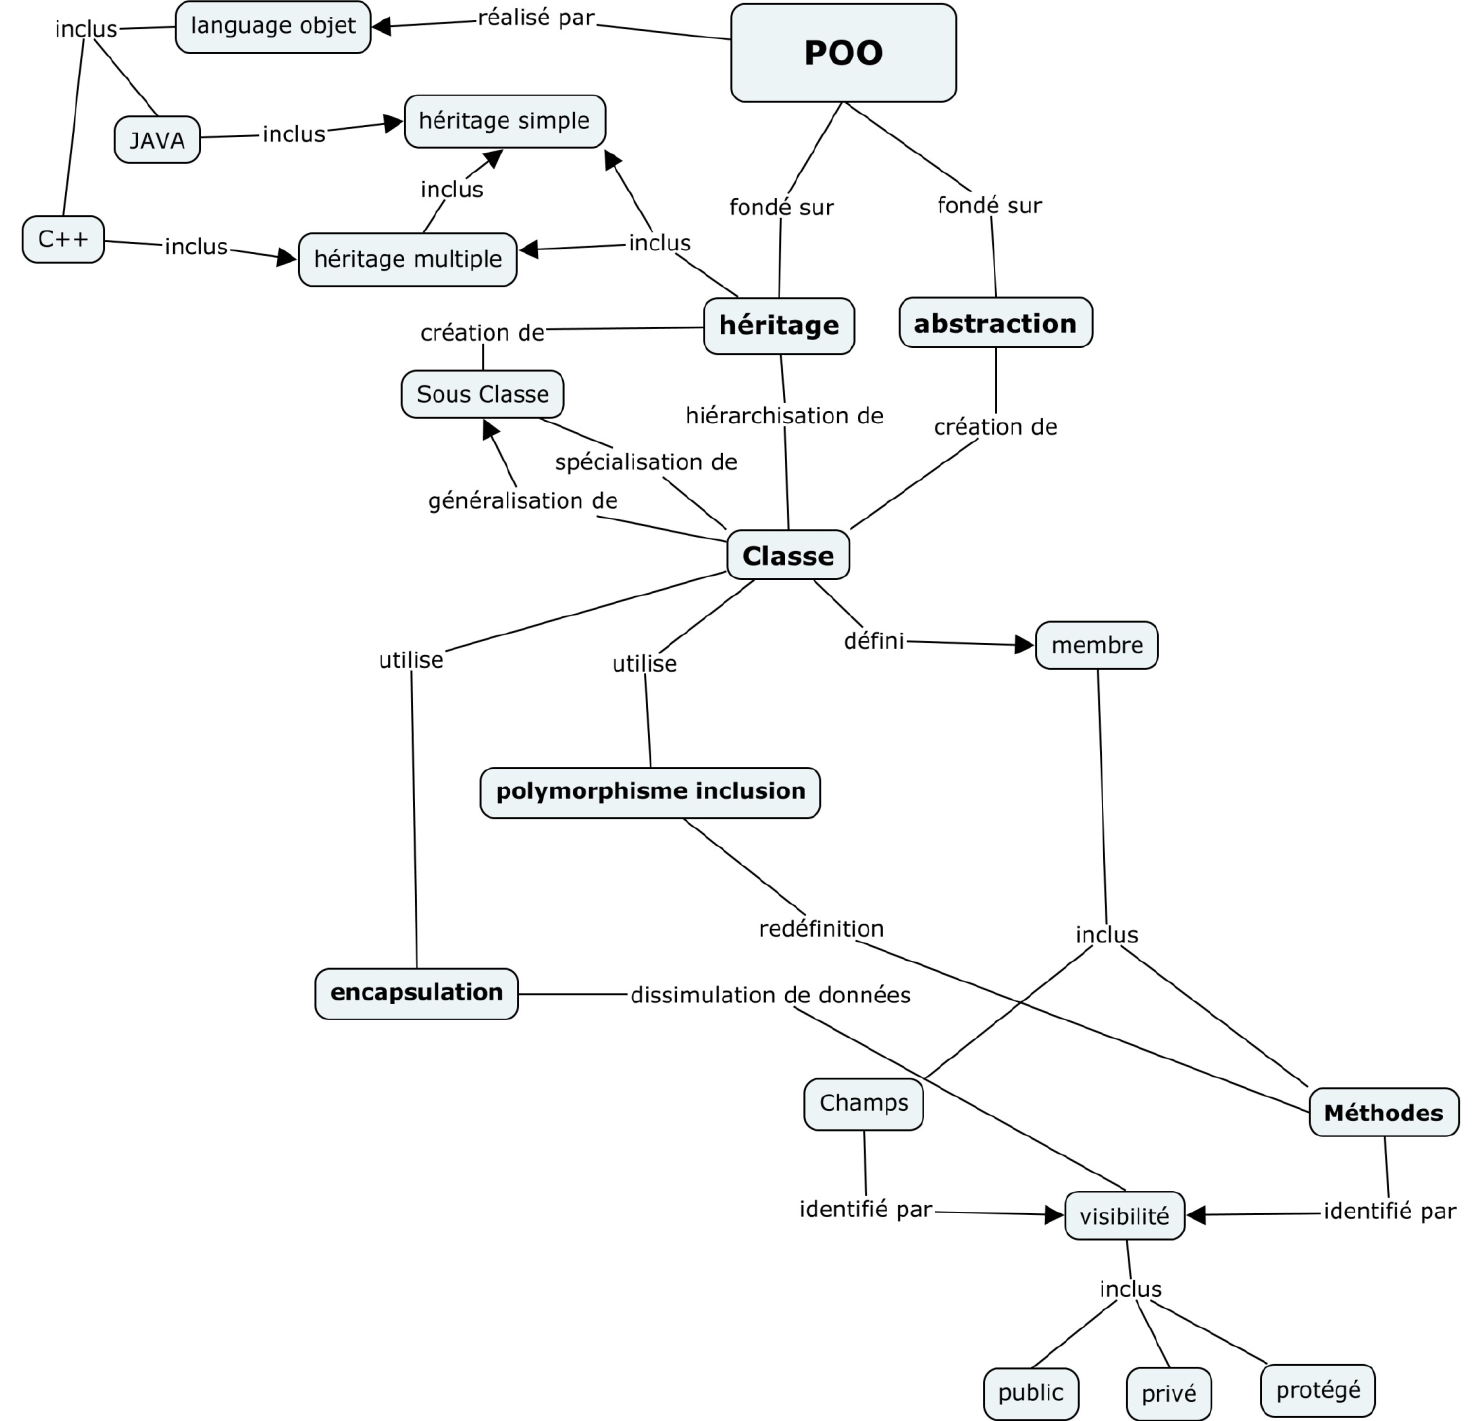
\includegraphics[scale=0.4]{resume2}

\end{document}

